\documentclass{article}

\usepackage{graphicx}
\usepackage{geometry}
\geometry{a4paper, scale=0.90}

\usepackage{CJKutf8}

\usepackage{caption}
\usepackage{subcaption}

\usepackage{wrapfig}
\usepackage{float}

\setlength{\parindent}{0em}

\usepackage{hyperref}

% Usage: \begin{Chinese}中文\end{Chinese}
\newenvironment{Chinese}
{\begin{CJK}{UTF8}{gbsn}}
{\end{CJK}}

\title{Numerical Analysis Homework-2 Submission}
\author{Zhuo Cheng (\begin{Chinese}程卓\end{Chinese}2021011617)}

\begin{document}

\maketitle

\section{Begin}

Code could be viewed on Github: 
\url{https://github.com/zhuocheng2004/Numerical-Analysis-2023/tree/main/HW2}

Below are various figures and some notes.

All written materials are presented at the end of this document.

\section{Problem 2}

Figure h -- Error:

\begin{figure}[H]
    \centering
    \begin{subfigure}[b]{0.8\linewidth}
	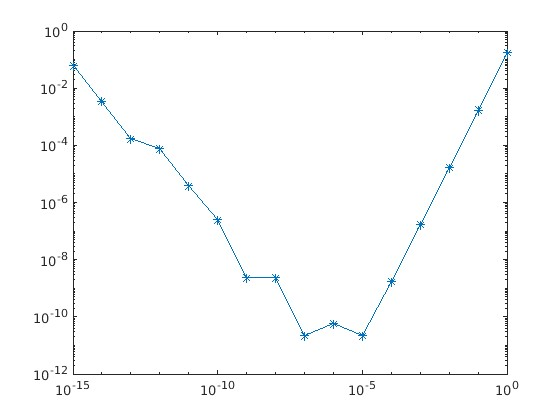
\includegraphics[width=\linewidth]{hw2_2_2.jpg}
        \caption{h -- error}
    \end{subfigure}
\end{figure}

\section{Problem 4}

\begin{figure}[H]
    \centering
    \begin{subfigure}[b]{0.3\linewidth}
	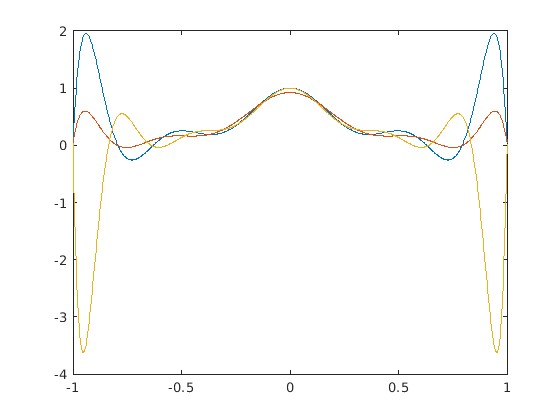
\includegraphics[width=\linewidth]{f1_equi_runge.jpg}
        \caption{Equidistant $10 \le N \le 12$ (Runge)}
    \end{subfigure}
    \begin{subfigure}[b]{0.3\linewidth}
	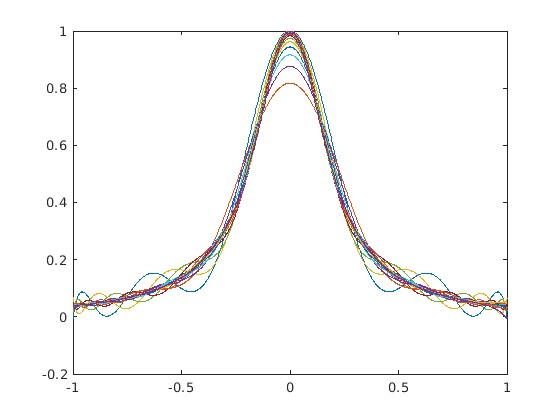
\includegraphics[width=\linewidth]{f1_cheb.jpg}
        \caption{Chebyshev $10 \le N \le 34$}
    \end{subfigure}
    \begin{subfigure}[b]{0.3\linewidth}
	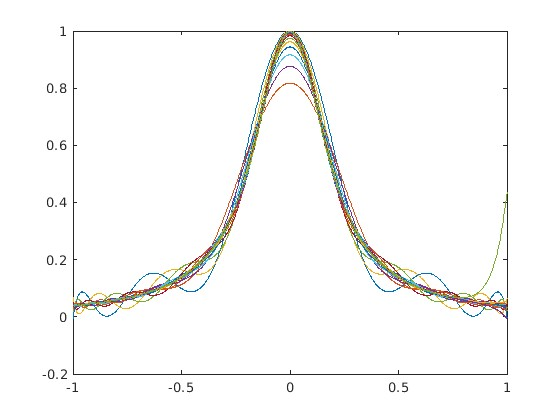
\includegraphics[width=\linewidth]{f1_cheb_1.jpg}
        \caption{Chebyshev $10 \le N \le 35$ (Runge?)}
    \end{subfigure}
    \caption{$f(x) = 1 / (1 + 25 x^2)$}
\end{figure}

\begin{figure}[H]
    \centering
    \begin{subfigure}[b]{0.4\linewidth}
	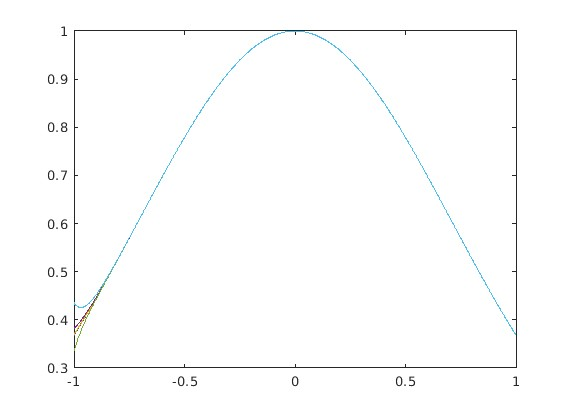
\includegraphics[width=\linewidth]{f2_equi.jpg}
        \caption{Equidistant $10 \le N \le 29$}
    \end{subfigure}
    \begin{subfigure}[b]{0.4\linewidth}
	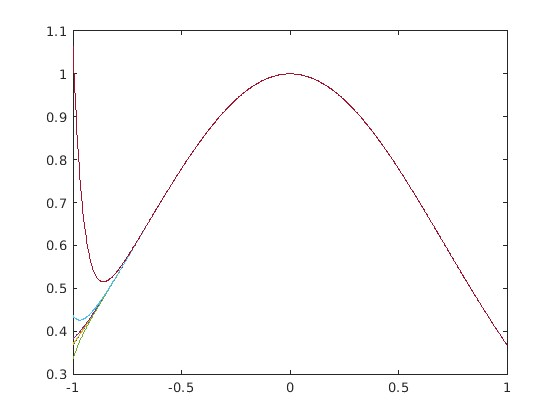
\includegraphics[width=\linewidth]{f2_equi_runge.jpg}
        \caption{Equidistant $10 \le N \le 30$ (Runge?)}
    \end{subfigure}
    \begin{subfigure}[b]{0.4\linewidth}
	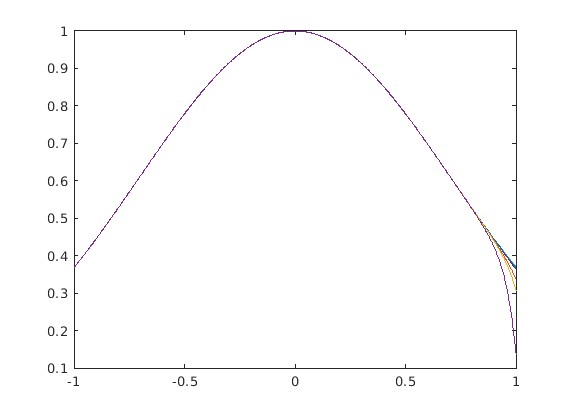
\includegraphics[width=\linewidth]{f2_cheb.jpg}
        \caption{Chebyshev $10 \le N \le 34$}
    \end{subfigure}
    \begin{subfigure}[b]{0.4\linewidth}
	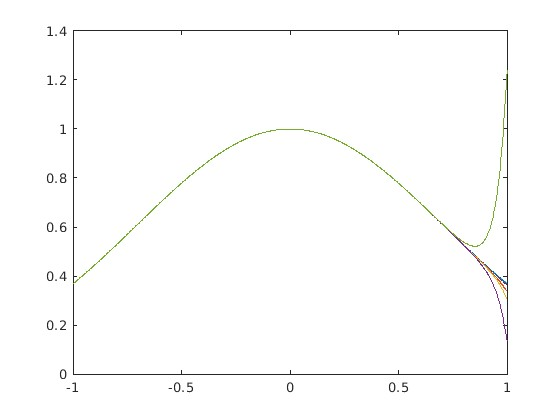
\includegraphics[width=\linewidth]{f2_cheb_1.jpg}
        \caption{Chebyshev $10 \le N \le 35$ (Runge?)}
    \end{subfigure}
    \caption{$f(x) = e^{-x^2}$}
\end{figure}

Error:

\begin{figure}[H]
    \centering
    \begin{subfigure}[b]{0.4\linewidth}
	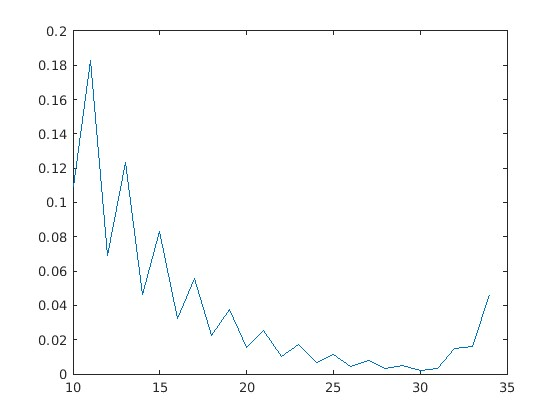
\includegraphics[width=\linewidth]{f1_error.jpg}
        \caption{$f(x) = 1 / (1 + 25 x^2)$ $10 \le N \le 34$}
    \end{subfigure}
    \begin{subfigure}[b]{0.4\linewidth}
	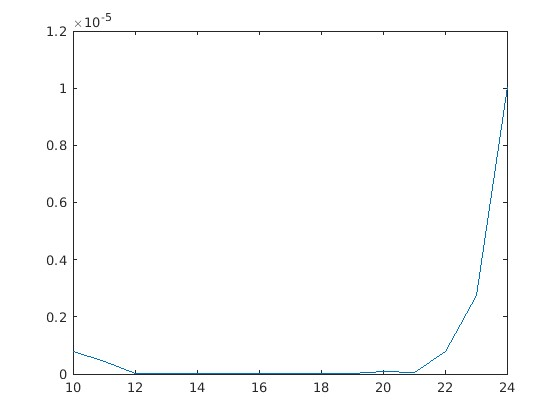
\includegraphics[width=\linewidth]{f2_error.jpg}
        \caption{$f(x) = e^{-x^2}$ $10 \le N \le 24$}
    \end{subfigure}
\end{figure}

These error results are quite strange and are not the ones shown in the class. 
Maybe I did something wrong.

It seems that for the first function, the minimal error was found near $N=30$.

For the second function, the error is mush smaller
(probably because the second function is more "smooth" than the first?), 
but the error increases rapidly as $N$ gets larger than 20. (Why?)

\section{Written Materials}

\begin{figure}[htbp]
	\centering
	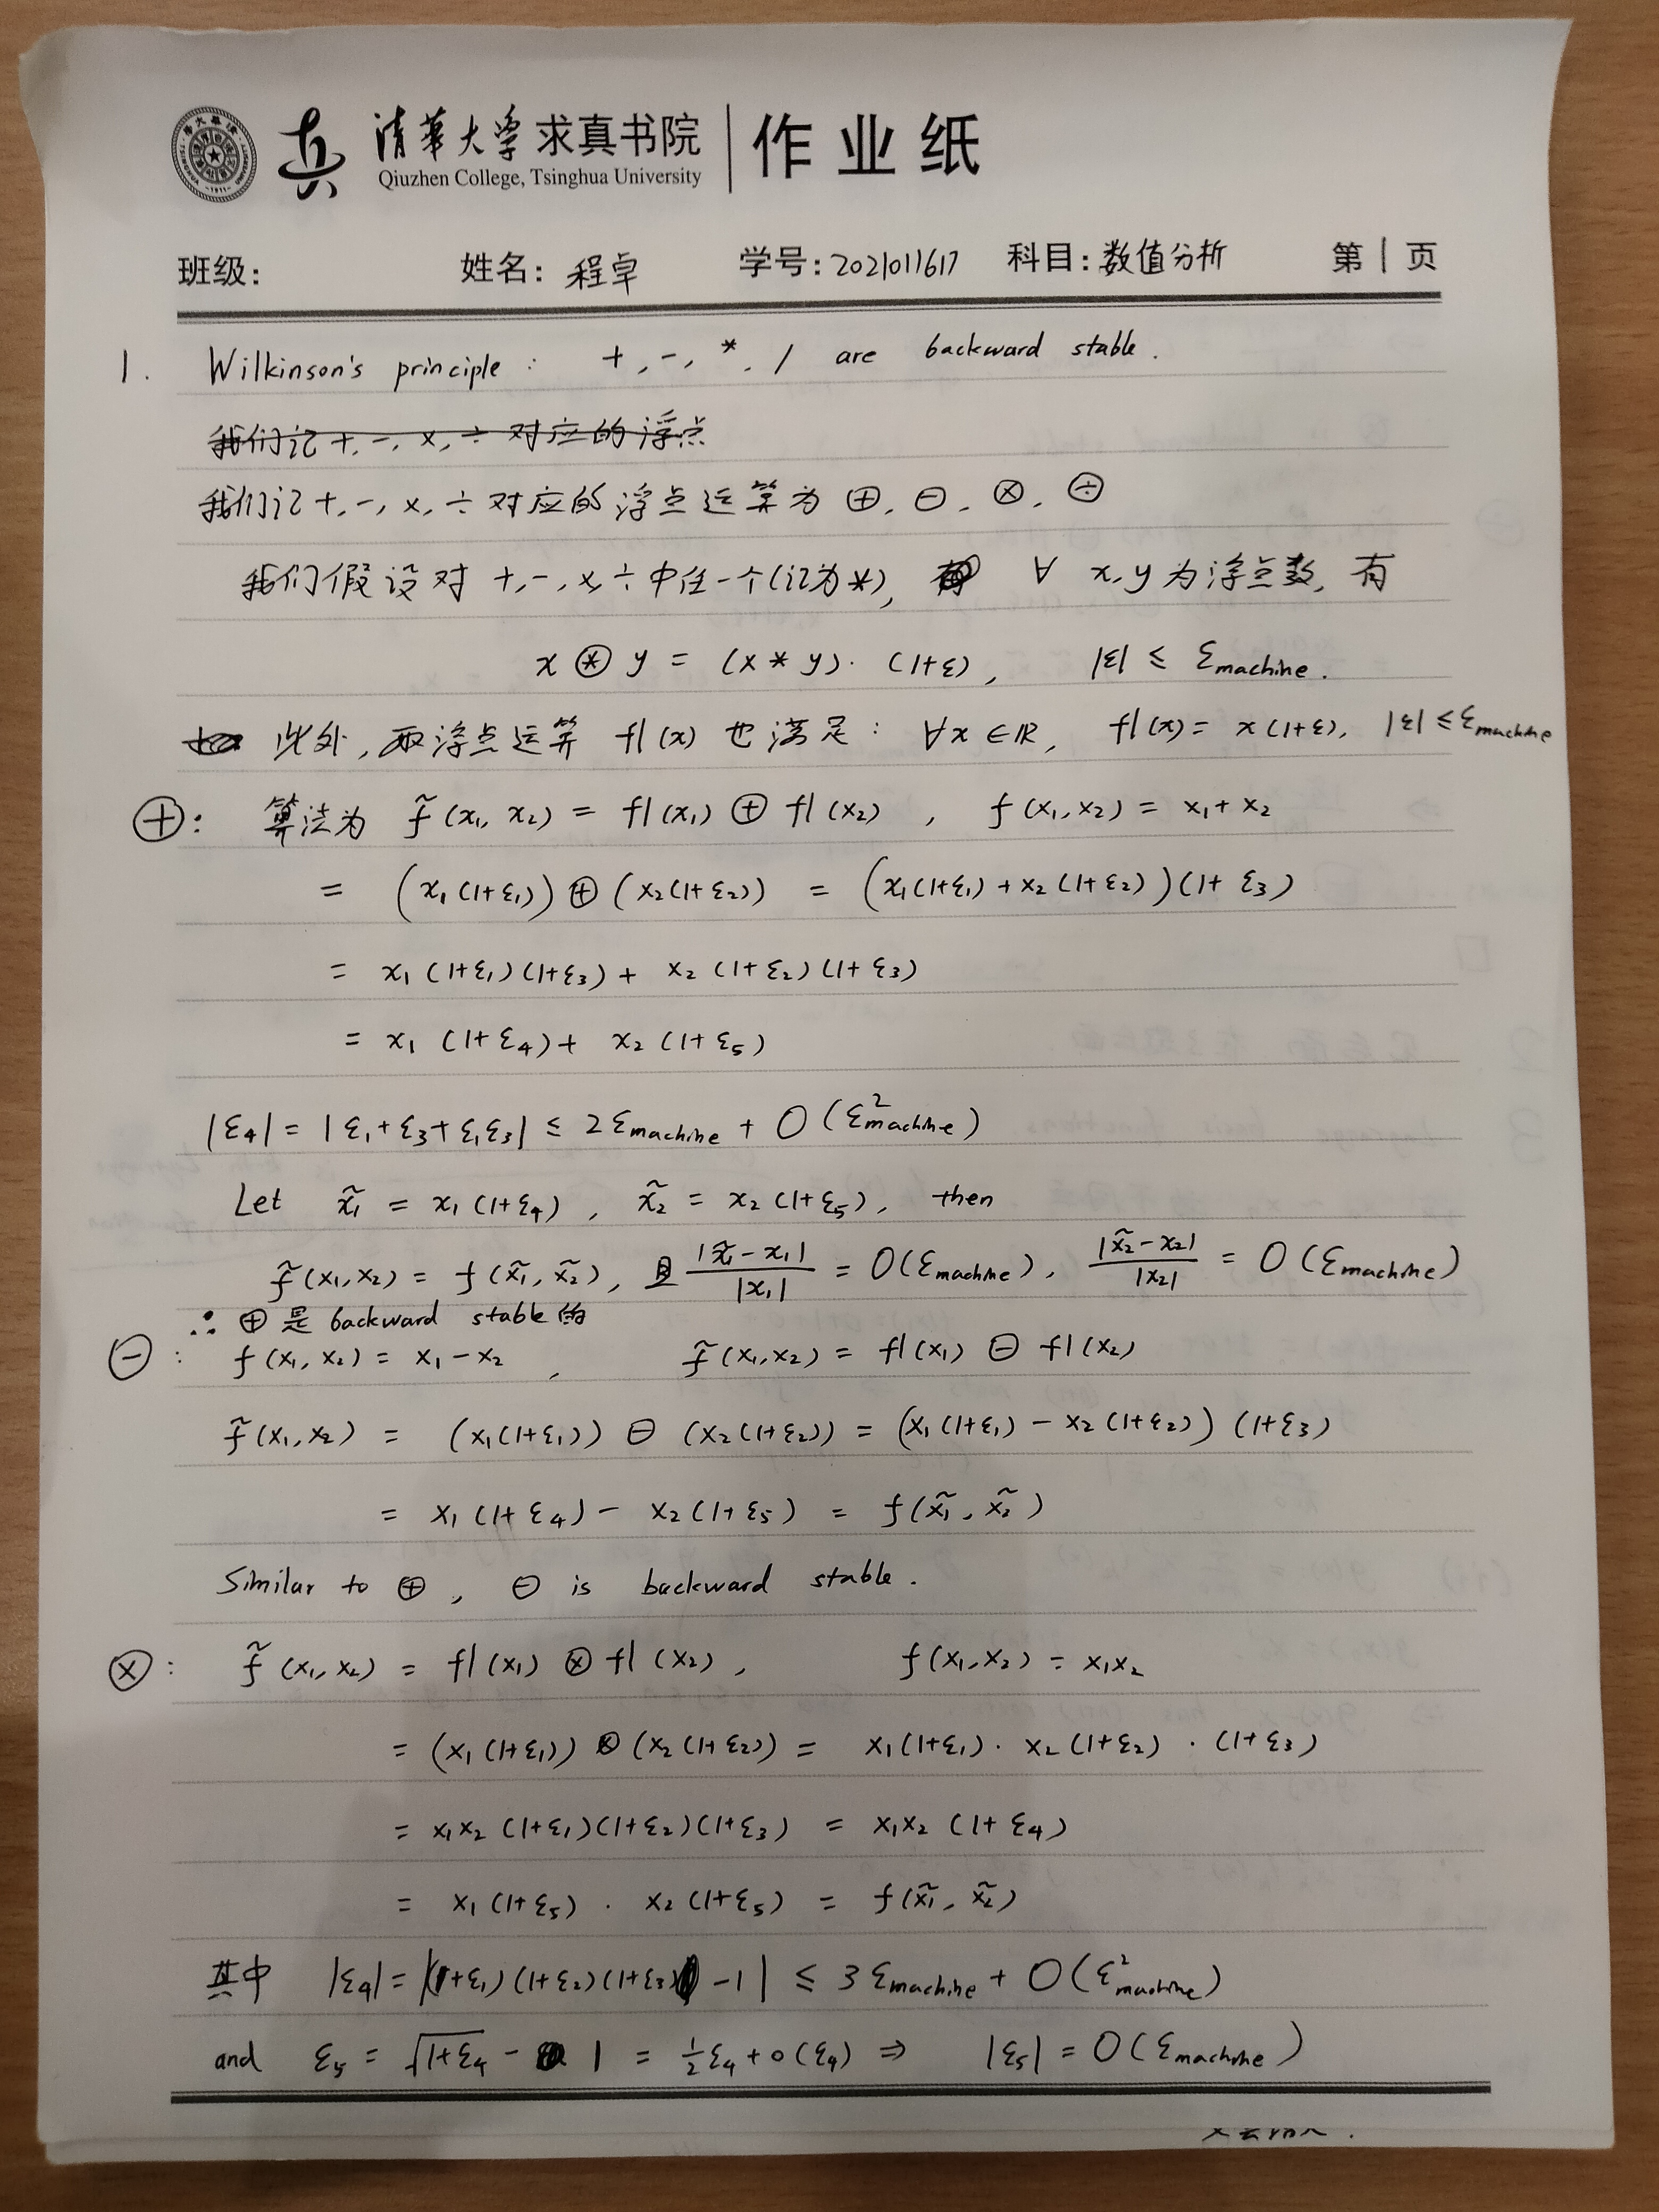
\includegraphics[width=\textwidth]{hwna0201.jpg}
\end{figure}

\begin{figure}[htbp]
	\centering
	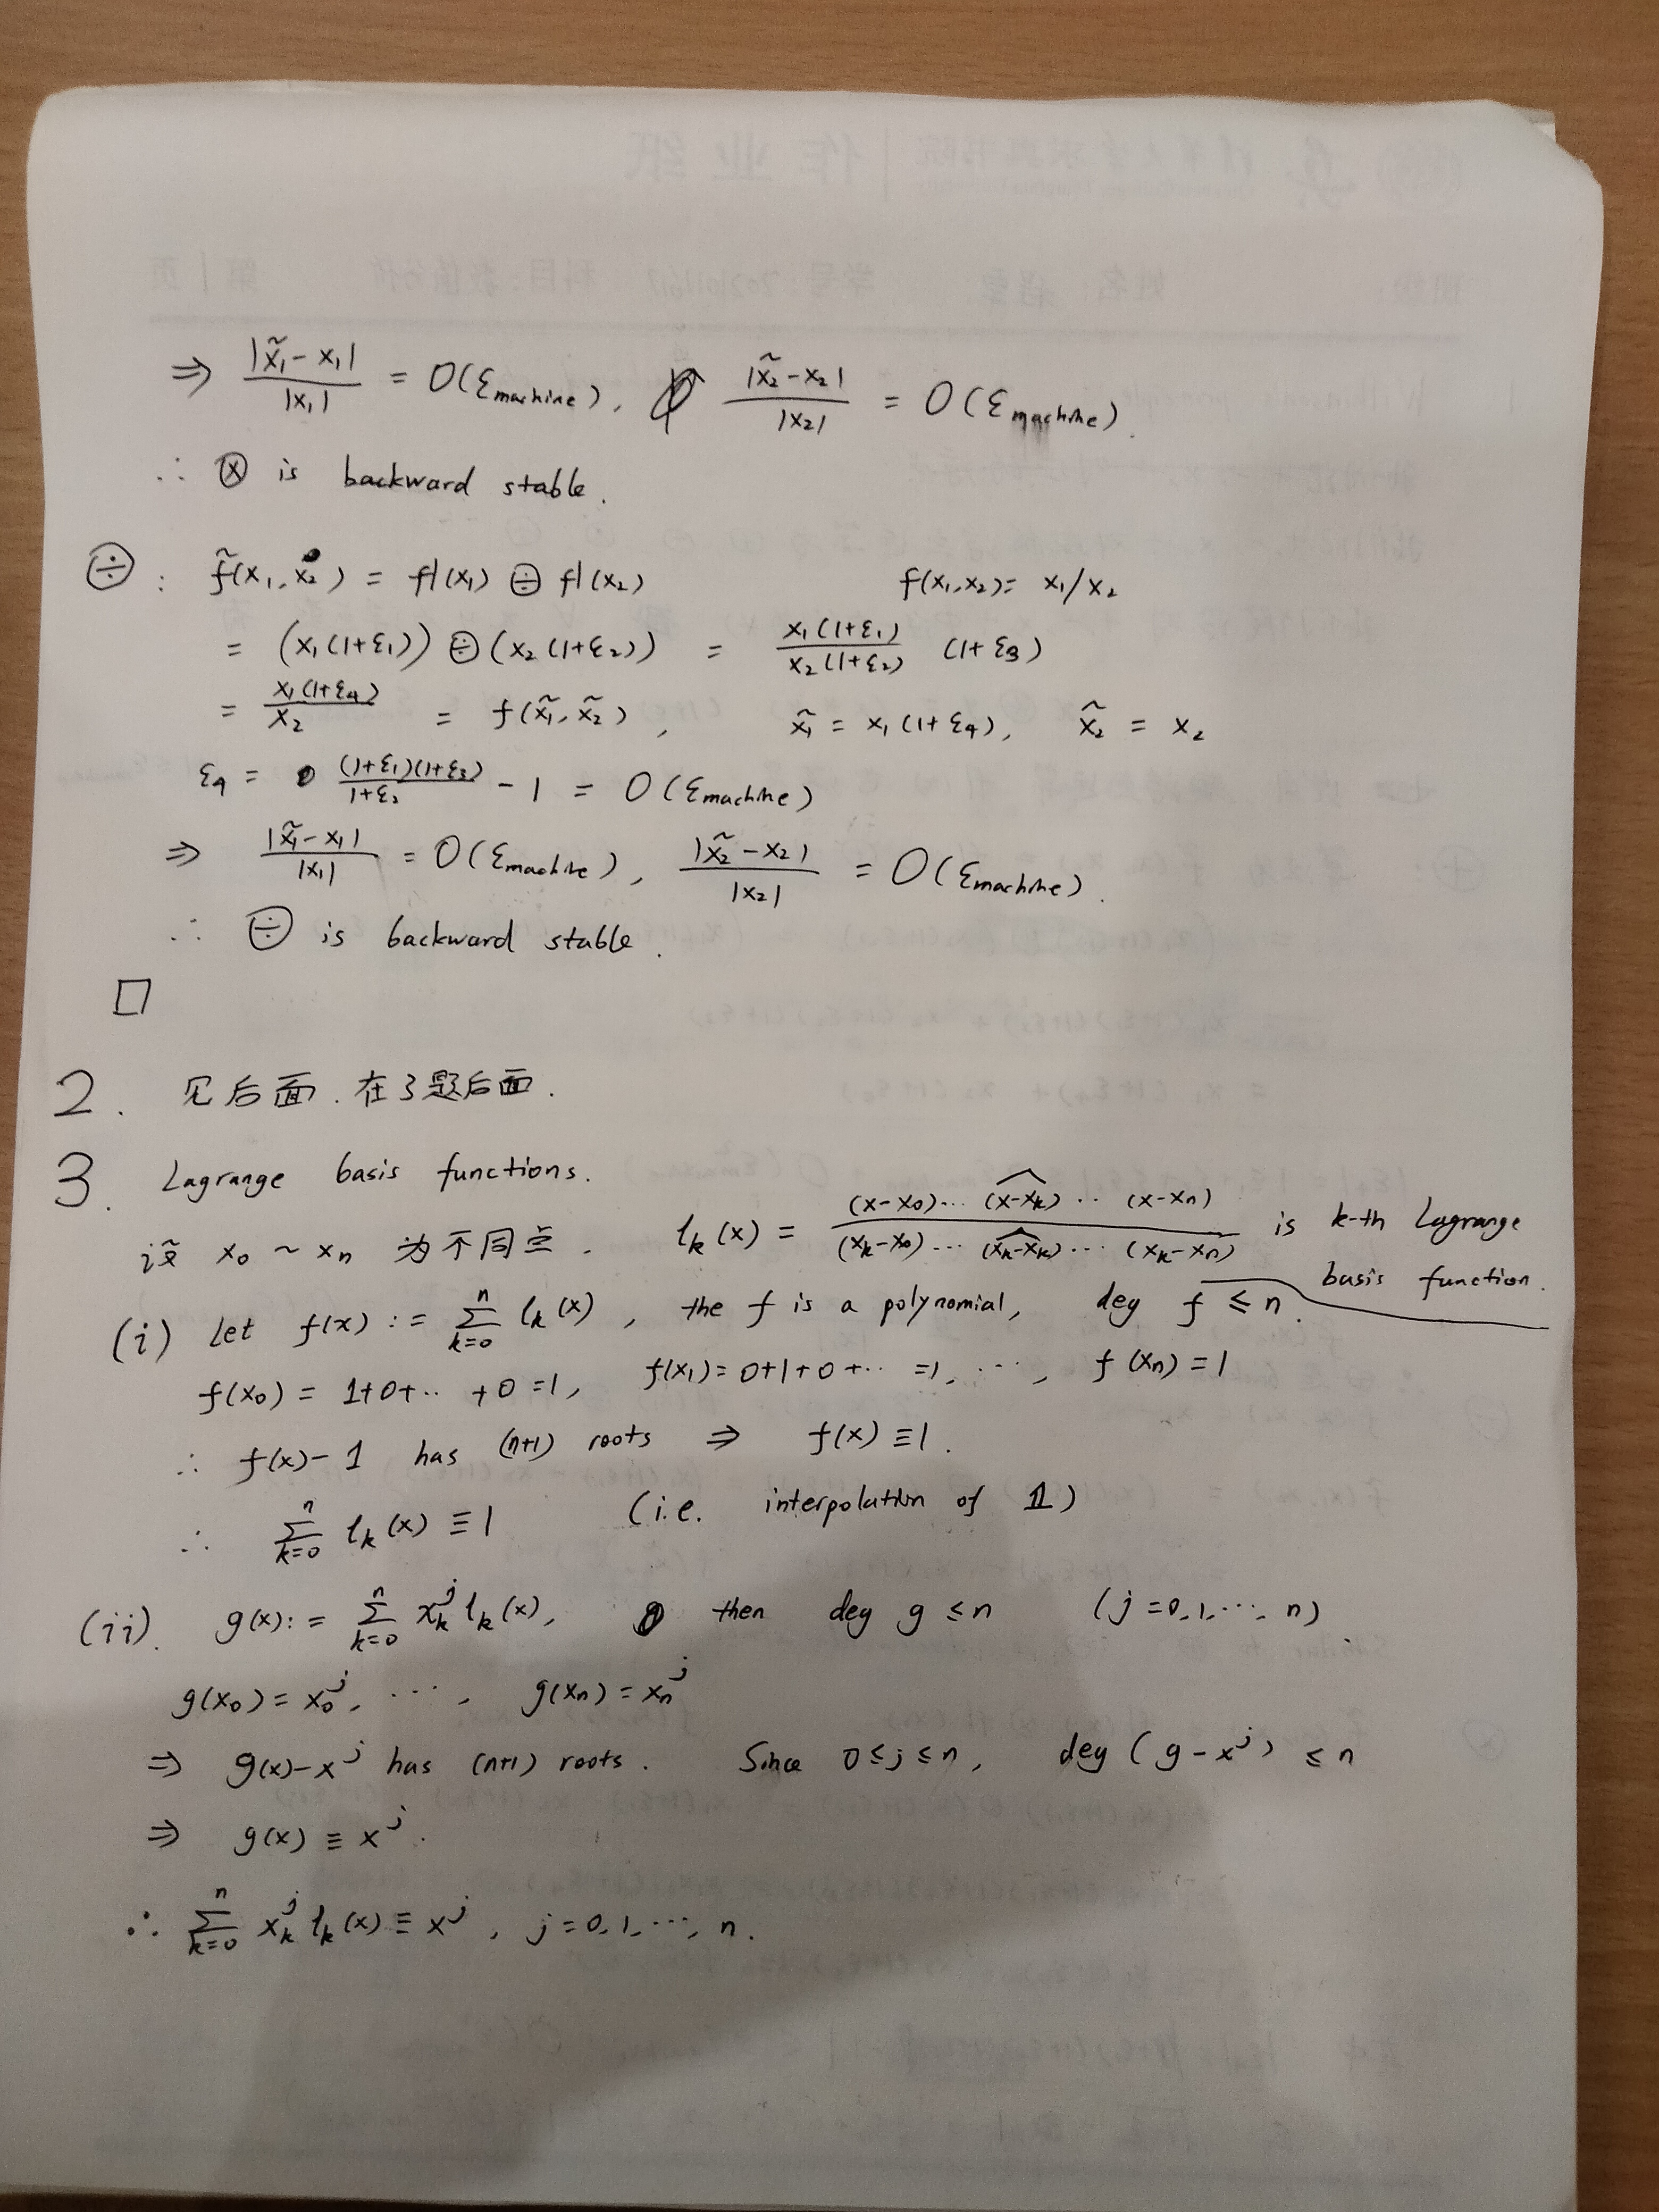
\includegraphics[width=\textwidth]{hwna0202.jpg}
\end{figure}

\begin{figure}[htbp]
	\centering
	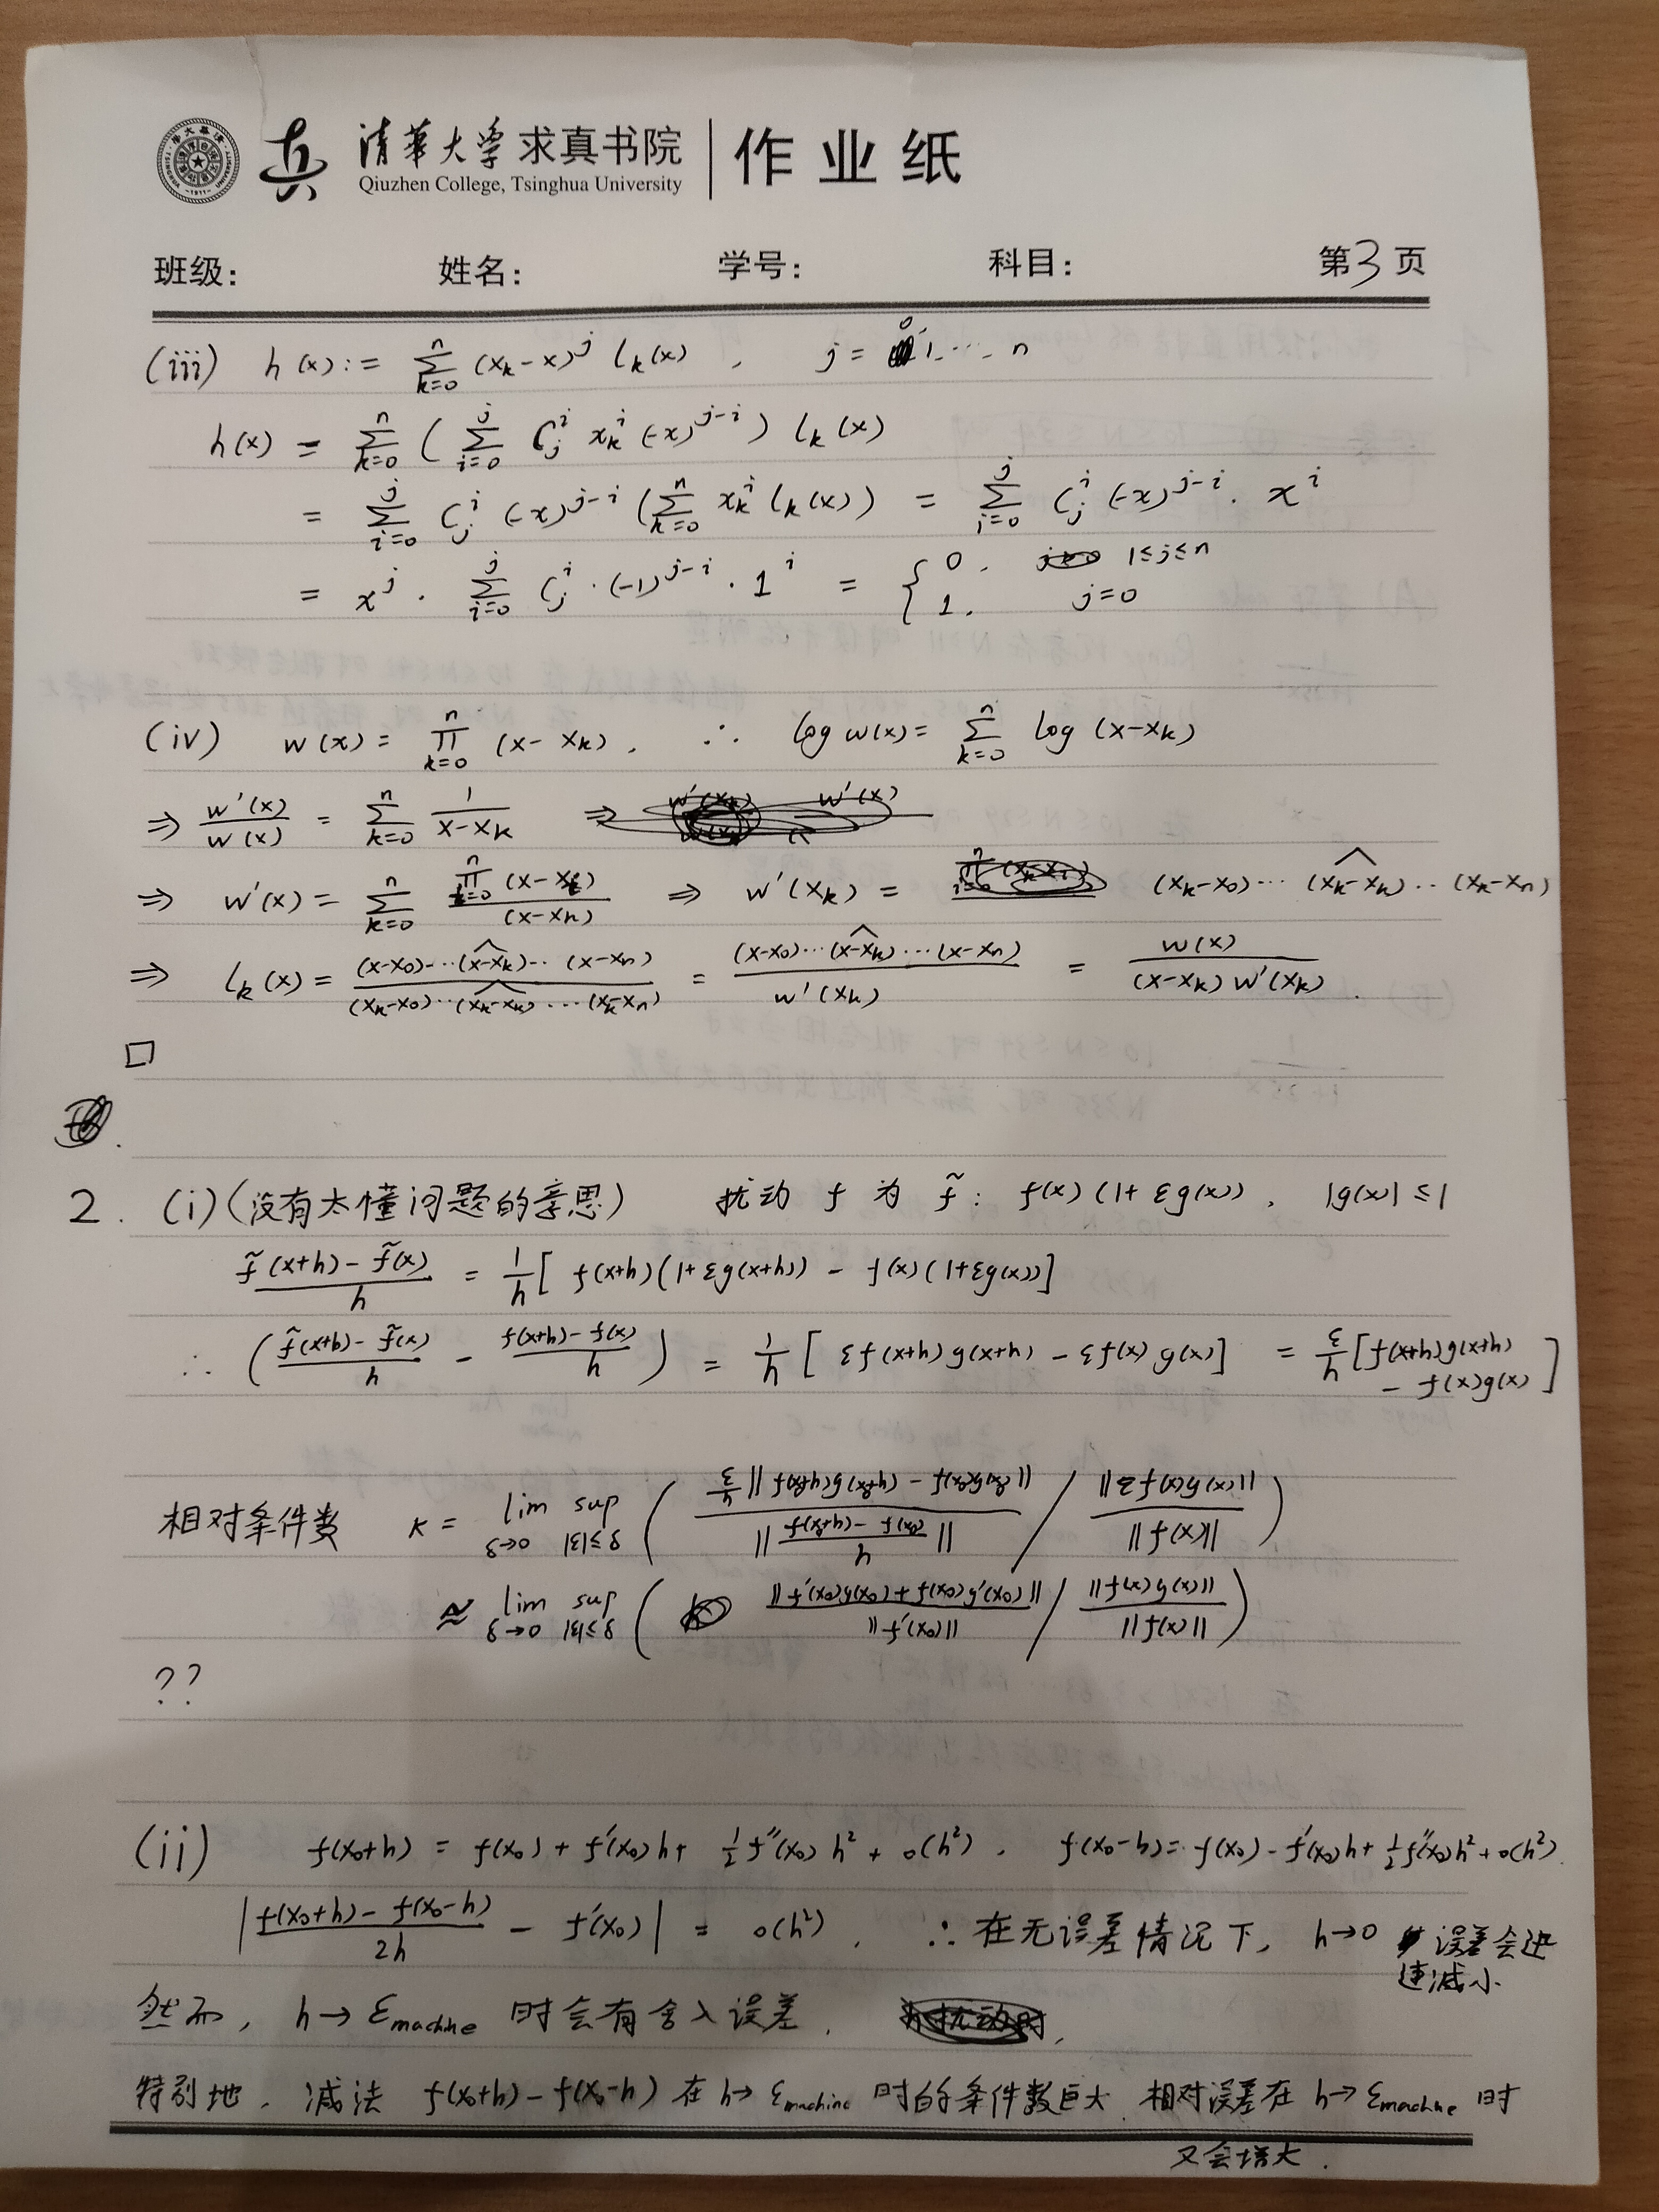
\includegraphics[width=\textwidth]{hwna0203.jpg}
\end{figure}

\begin{figure}[htbp]
	\centering
	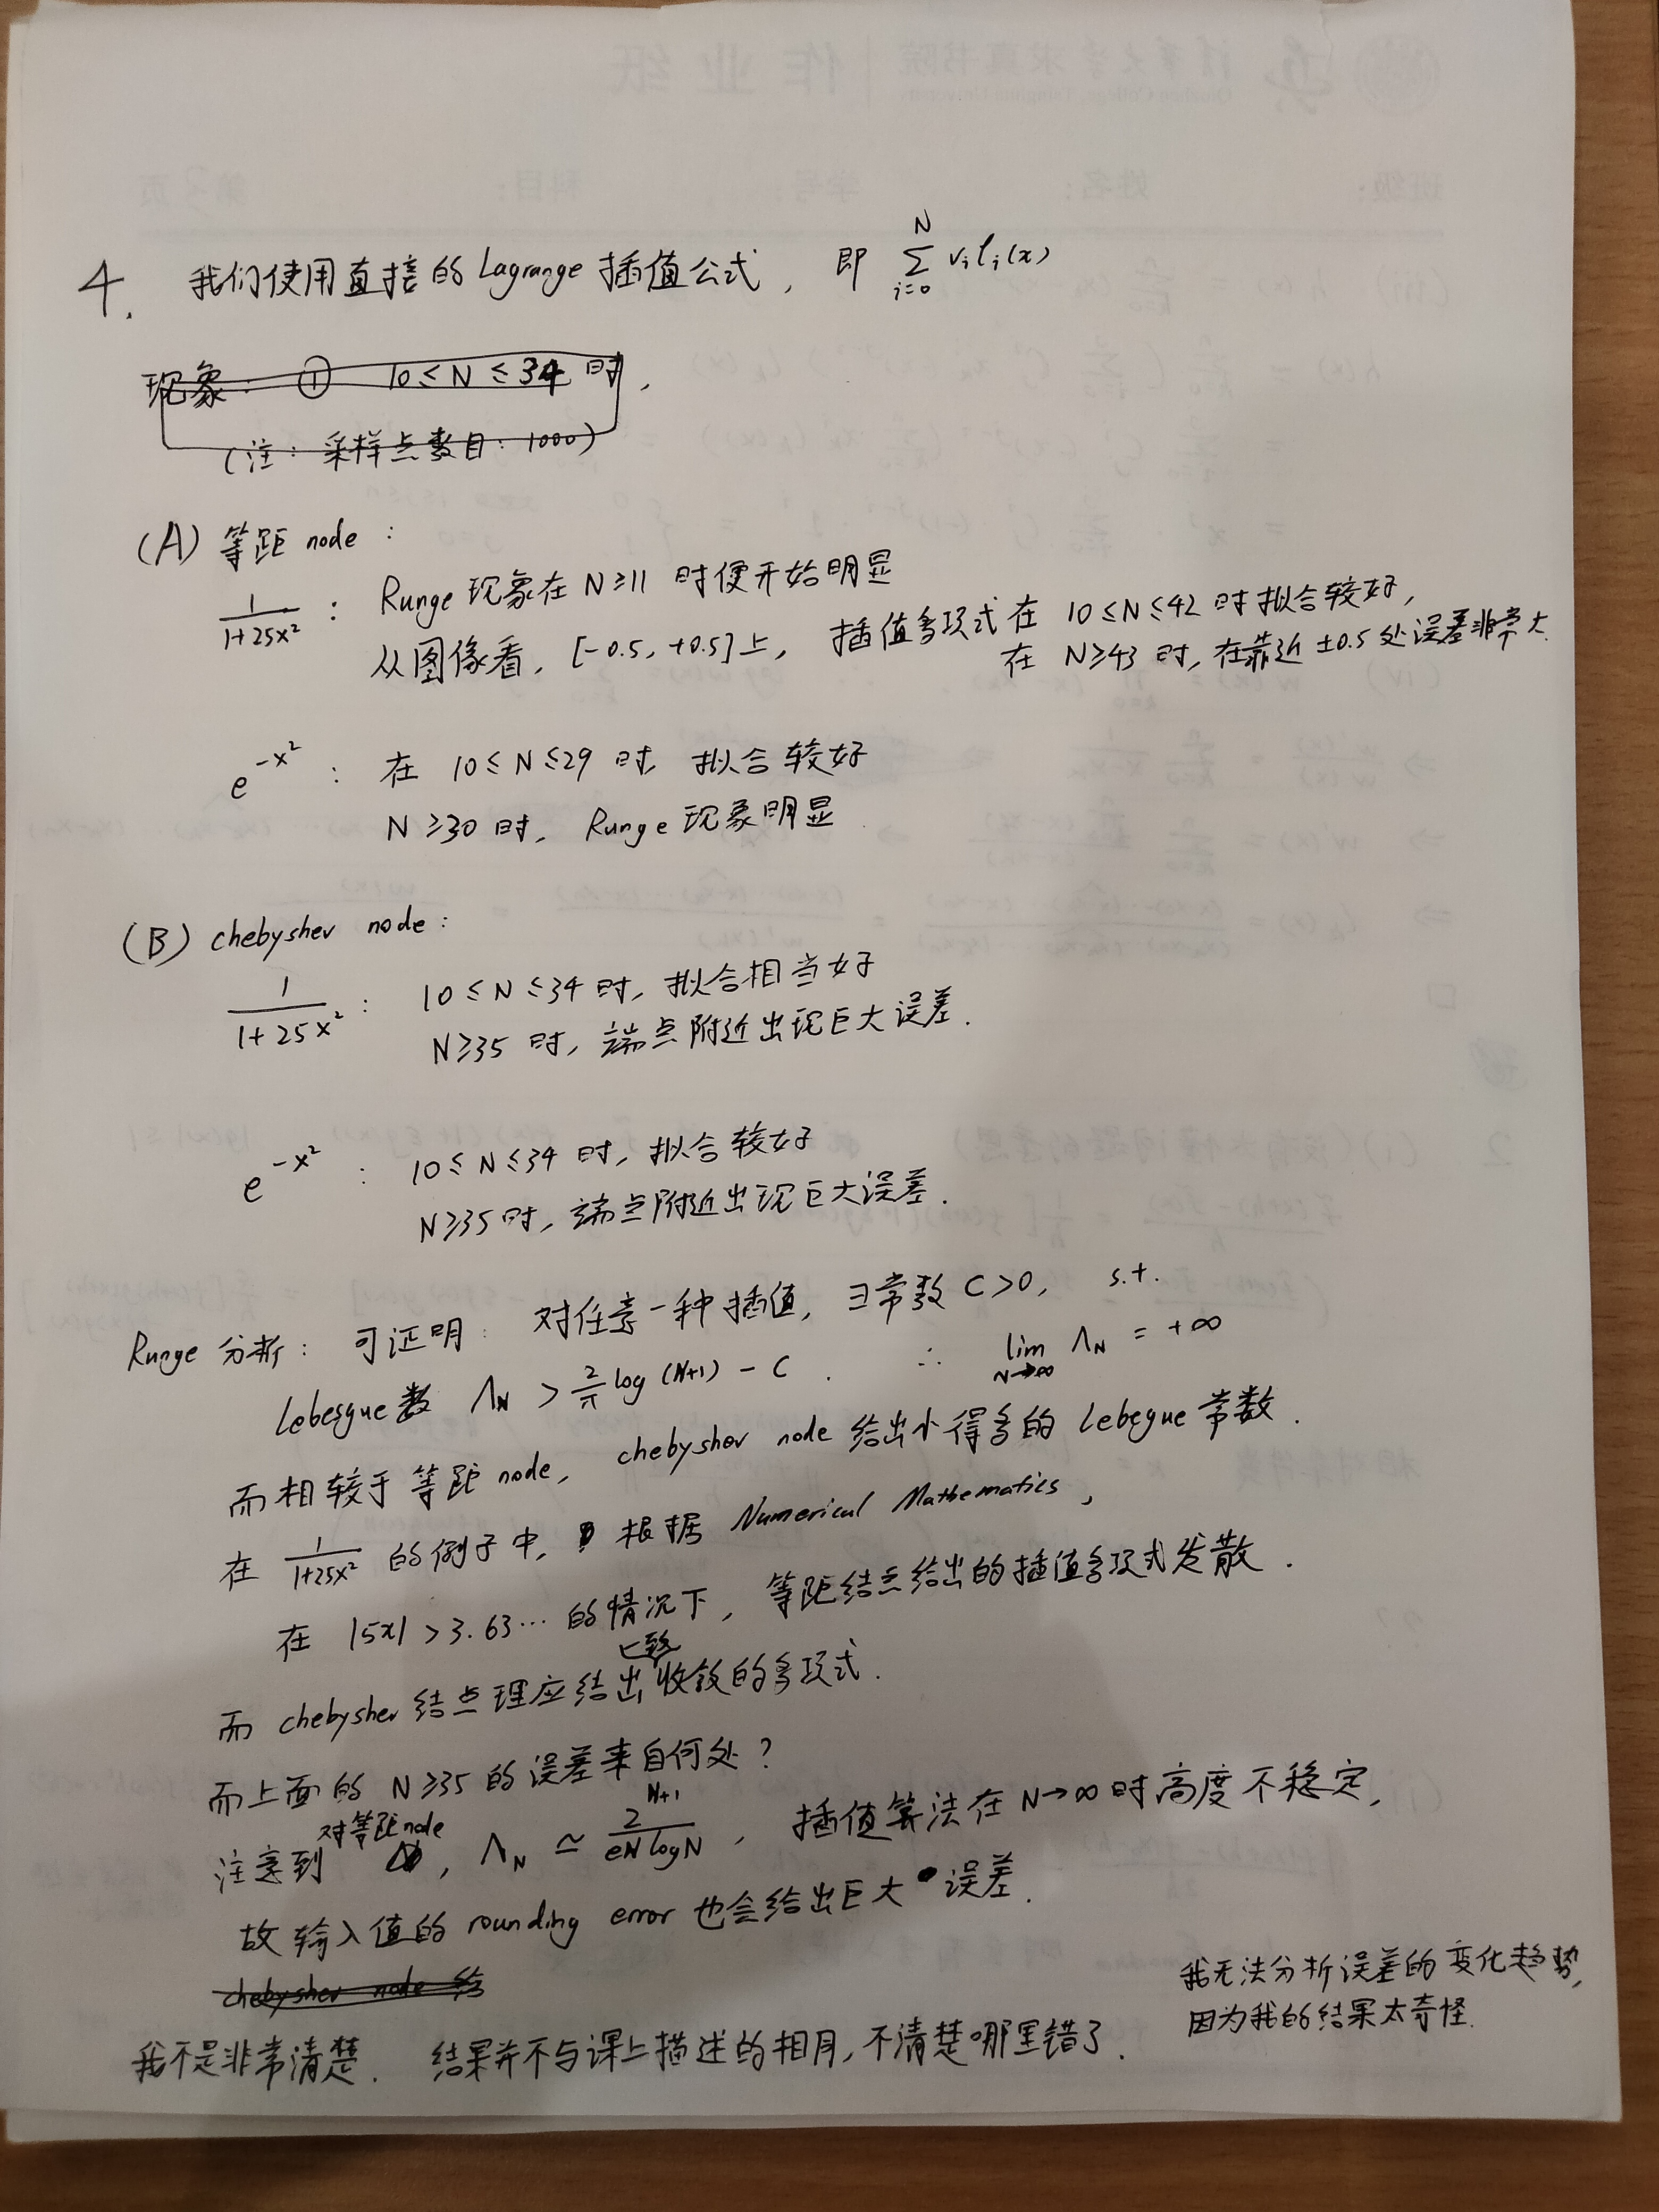
\includegraphics[width=\textwidth]{hwna0204.jpg}
\end{figure}

\end{document}

